\section{Umsetzung}
\subsection{Lösungsansatz} 
Für die Umsetzung des Chatprogramms wird die Peer-to-Peer Architektur verwendet. 
Ziel ist die Entwicklung einer Chatanwendung, die keine weiteren Infrastrukturkomponenten benötigen.
Dadurch kann der Chatroom jederzeit in jedem Netzwerk eröffnet und verwendet werden, ohne zusätzliche Voraussetzungen. 
\\
Die Applikation soll es ermöglichen, dass mehrere Nutzer im selben Netzwerk miteinander chatten können. 
Dafür müssen zu Beginn andere Teilnehmer im Netzwerk gefunden werden, es wird eine Art Service discovery benötigt.
Es gibt verschiedene Möglichkeiten andere Services zu finden. 
Zum einen kann ein Broadcast verwendet werden.
Multicast routing hingegen sendet ein Paket an eine definierte Empfängergruppe. 
Die Bandbreite des Netzwerks wird hierbei besser und effizienter genutzt\cite[S. 382f]{tan10}.
Dennoch wird auch hier das Wissen über alle vorhandenen Adressen benötigt\cite[S. 381]{tan10}. 
Durch die Kombination von dns und multicast routing ist es möglich eine bestimmte Empfängergruppe in einem Netzwerk zu addressieren. 
Da jederzeit neue Teilnehmer hinzukommen können und den Chatroom wieder Verlassen können, wird eine Service discovery Methode benötigt, die es ermöglicht durchgehend andere User zu finden und gefunden zu werden.
MDNS ermöglicht jederzeit das Finden von anderen Benutzern und das dauerhafte Warten auf die Bekanntgabe eines neuen Users\cite[S. 611f]{tan10}. 
Da mDNS nicht geroutet wird, bleibt die Suche im selben Netzwerk und ist geeignet für die Suche anderer Teilnehmer in dieser Applikation.
Da kein Server angefragt werden kann und nur Geräte adressiert werden sollen, die Teil des lokalen Netzwerks sind, bietet sich mdns an\cite[S. 382]{tan10}. 
Für die Verwendung des Chatrooms muss im Vorhinein identifiziert werden, welche Teilnehmer zu der zu addressierenden Gruppe gehören. 
\\
\\
Wurde ein Chatteilnehmer gefunden, muss herausgefunden werden, wer der Teilnehmer ist. 
Es wird ein Merkmal benötigt, was nur einmalig vorhanden ist und womit ein User sicher im Netzwerk identifiziert werden kann. 
Jedem Computer ist eine eigene IP Adresse zugewiesen, die nur einmal im Neztwerk auftauchen kann. Anhand dieser Adresse kann ein Teilnehmer im Neztwerk identifiziert werden.
Der User kann allerdings nur mit der IP Adresse der anderen Teilnehmer nicht wissen, wer die anderen Personen im Chatroom sind. 
Somit muss sowohl die Adresse, als auch der Name des jeweils anderen herausgefunden und gespeichert werden. 
In Form einer Hallo-Nachricht kann der eigene Name und die IP Adresse bekannt gegeben und an die gefundenen Nutzer gesendet werden. 
Um zu wissen welcher User zu der gefundenen IP Adresse gehört, wird auf die eigene Hallo-Nachricht ebenfalls mit einer Hallo-Nachricht geantwortet. 
Die gefundenen IP Adressen müssen gespeichert werden, damit jeder Client weiß, welche anderen Clients momentan Teil des Chatrooms sind. 
Zur Speicherung der gefundenen User wird eine Liste angelegt. Somit weiß jeder Nutzer welche anderen Teilnehmer vorhanden sind. 
Nachdem herausgefunden wurde, welche Nutzer da sind, muss nicht mehr aktiv nach Teilnehmern gesucht werden. 
Dennoch muss es weiterhin möglich sein, von neuen Teilnehmern gefunden zu werden, wodurch ein Service benötigt wird, der dauerhaft das eigene Gerät im Netzwerk listet.
\\
\\
Nach dem Chatroombeitritt können Nachrichten verschickt werden. 
Neben dem Schreiben von Nachrichten sollen auch Nachrichten von anderen empfangen werden. 
Somit müssen mehrere Prozesse gelichzeitig stattfinden, was zu einer Problematik führt. 
Der Computer agiert als Client und Server, um gleichzeitig Nachrichten zu senden und empfangen. 
Das Starten des Servers, als auch das Senden von Nachrichten sind blocking-calls, weshalb die Aktionen nicht gleichzeitig ablaufen können.
Sobald der Server gestartet ist und nach Teilnehmern sucht, kann kein anderer Prozess stattfinden. 
Der laufende Thread wird vom Server blockiert, wodurch es nicht möglich ist gleichzeitig Nachrichten zu versenden. 
Um dauerhaft zeitgleich Nachrichten empfangen als auch senden zu können, wird der Server in einen Thread ausgelagert. 
Ein Thread ist ein Ausführungsstrang eines Prozesses, der sich mit anderen Strängen Ressourcen teilt.
Threads haben einen Programmcounter um zu wissen, welche Aktion als nächstes ausgeführt werden muss. Des Weiteren besteht ein Thread aus Registern, um die derzeitigen benutzten Variablen zu halten und einem Stack, 
um die Historie von Ausführungen zu speichern\cite[S. 103]{tan15}. 
Damit können innerhalb eines Prozesses meherer Threads gleichzeitig laufen\cite{multithreading_2017}. 
Threads sind einfacher zu erstellen und auch wieder zu beenden als ganze Prozesse. Deswegen bietet sich multithreading in Situationen an, in denen mehrere Abläufe gleichzeitig stattfinden sollen\cite[S. 98]{tan15}
Eine ähnliche Prolematik stellt sisch auch bei der Service discovery. Diese kann genauso mit einem weiteren Thread gelöst werden. 
\\
\\
Da es sich um einen Chatroom handelt, sollen alle Teilnehmer alle gesendeten Nachrichten erhalten.
Durch die Verwendung von Client-Server Protokollen ist jedoch nur one-to-one Kommunikation möglich, weshalb die Nachrichten an jede vorhandene Adresse in der Liste verschickt werden müssen\cite[S. 214]{steen23}.
\\
\\
Bei Beendingung des Programms müssen die Teilnehmer über den Austritt informiert werden, damit keine weiteren Nachrichten an den User gesendet werden.
Verließe ein User den Chatroom, ohne andere Teilnehmer darüber zu informieren, würden weiterhin Nachrichten an seine Adresse geschickt werden, weil sie nie bei den anderen Teilnehmern aus der Liste entfernt wurde.
Es sollen keine weiteren Nachrichten an den austretenden Teilnehmer mehr zugestellt werden.
Deshalb muss mit dem Verlassen des Chatrooms sichergestellt werden, dass die anderen Geräte die Adresse aus ihren Listen löschen.
Durch das Versenden einer speziellen Nachricht mit den eigenen Daten beim Verlassen des Chatrooms, kann der Teilnehmer aus der Liste der anderen Peers gelöscht werden. 
Beim Austritt muss neben der Abmeldung auch der Server gestoppt werden, was automatisch mit dem Verlassen des Chatrooms einhergehen soll. 
Anschließend ist die Chatapplikation beendet.
\subsection{Technische Entscheidungen}
Die Anwendung wurde in Python geschrieben. Für das Versenden von Nachrichten werden HTTP requests genutzt und eine REST API. Hierbei wurde sich für die Nutzung von FastAPI entschieden\cite{fastapi}. 
Das Programm wurde in verschiedene Abschnitte gegliedert und orientiert sich am Model-View-Controller Pattern. 
Damit wird das Programm in drei große Kategorien unterteilt. 
Model bezieht sich auf die Daten, View präsentiert die Modeldaten dem User und Controller verarbeitet Userinput und updatet sowohl Model als auch View.
In diesem Projekt finden nur die Kategorien Model und Controller Anwendung, da die Modeldaten dem User nicht präsentiert werden müssen.
Dies ermöglicht eine klare Trennung der verschiedenen Zuständigkeiten und erleichtert die Wartung, sowie die Erweiterung des Programms.
\subsubsection{API}
Das application programming interface, genannt API, ist ein Interface, welches aus libary calls besteht\cite[S. 129]{steen23}.
Eine spezielle und häufig genutzte Form der API ist die REST API.
Die Representational State Transfer API zeichnet sich durch verschiedene Charakteristiken aus.
Bei der  REST API werden Ressourcen durch ein vorgegebenes Namensschema identifiziert. Das dabei benutzte Protokoll ist HTTP.
Auf Anfragen von Informationen werden mittels Anwesiungen die gewünschten Informationen zurückgegeben. Dabei wird eine der vier Operationen 
in Kombination mit der URI verwendet\cite[S. 66f]{steen23}. 
Außerdem bieten alle Services die selben Interfaces an, welche aus vier Operationen bestehen, die ausgeführt werden können. 
Die \emph{PUT} Operation wird verwendet, um eine bereits vorhandene Ressource zu verändern.\emph{POST} wird für die Erstellung einer neuen Ressource benötigt.
Für Informationen über vorhandene Ressourcen wird die Operation \emph{GET} verwendet und \emph{DELETE} findet Anwendung wenn eine Ressource gelöscht werden soll.
Des Weiteren sind die versendeten Nachrichten von verschiedenen Services über REST selbsterklärend.
Wurde eine Anfrage bearbeitet und eine Operation ausgeführt, wird keine Information über den Anfrager gespeichert. 
Somit wird ein HTTP request verschickt, um die benötigten Daten zu bekommen. 
Je nach Anfrage kann eine error Message zurückgegeben werden, falls die Anfrage fehlgeschlagen ist. 
Schlägt die Anfrage nicht fehl, werden die angefragten Daten als Antwort zurückgegeben. 
Die einzelnen Applikationen können alle geforderten Informationen mittels der wenigen Operationen erhalten\cite[S.67 ]{steen23}. 
Durch diese Simplizität der Architektur von REST ist es eine einfache Lösung für komplizierte Kommunikationskonzepte.
REST bietet die Möglichkeit mit einem standardisierten Set von HTTP Verben Abfragen durchzuführen, sodass in gleichen Situationen auch die gleiche Operation ausgeführt wird.
Für den Chat Client bietet die Verwendung von einer REST API die Möglichkeit, Nachrichten an einen bestimmten Endpunkt zu schicken und zu definieren, welcher Antworttyp zurückgegeben werden soll.
Betrachtet man das Richardson Maturity Model ist zu sehen, dass die Verwendung der REST API in diesem Projekt sich an den Konzepten des Modells orientiert\cite{richardson}. 
Die REST API arbeitet ebenfalls mit HTTP Requests und durch den Einsatz von Statuscodes wird direkt angezeigt, welches Ergebnis der gewünschte Request bringt. 
% richardson maturity model, welches level und warum 
% warum nutze ich Rest? 
\subsection{Komponenten} 
Für die einzelnen Aufgaben der Anwendung werden verschiedene Komponenten benötigt, sowohl aktive als auch passive. Jede vorhandene Komponente übernimmt eine bestimmte Aufgabe der Chatanwendung. 
Durch die Aufteilung entsteht eine Ordnung und Struktur innerhalb des Programms. Dies ermöglicht ein effizienteres und übersichtlicheres Datenmanagement.
Die Chat-Applikation setzt sich im wesentlichen zusammen aus:
\begin{itemize}
    \item DiscoveryService 
    \item Receiver
    \item Transmitter
    \item ConfigData
    \item Message types
\end{itemize} 
\subsubsection{DiscoveryService}
Um mit dem Chatten starten zu können wird der DiscoveryService benötigt. 
Er betreibt aktiv die Servicesuche über mdns und versendet die Startmessages an alle gefundenen Adressen. Die gefundenen Teilnehemr werden von dem DiscoveryService in die Userliste eingetragen. 
Anschließend fungiert er als mDNS responder um weiterhin von neuen Teilnehmern gefunden zu werden und diese in der Liste zu ergänzen. 
\subsubsection{Receiver}
Im Receiver werden die Messageendpunkte definiert, um die gesendeten Nachrichten über HTTP zu empfangen. 
Die Messages werden in der Konsole mit zugehörigem Namem ausgegeben.
Die HTTP Endpunkte werden mit FastAPI bereitgestellt. Der Receiver übernimmt außerdem die Verwaltung des benötigten Serverthreads.  
\subsubsection{Transmitter}
Der Transmitter ist verantwortlich für die Verarbeitung und den Versand der von Usern eingegebenen Nachrichten. 
In einer Dauerschleife nimmt er solange Nachrichten entgegen, bis \emph{exit} eingegeben wird. Die eingebenen Messages werden ebenfalls in der Konsole ausgegeben.
\subsubsection{ConfigData}
In der ConfigData ist die Userliste mit IP Adresse und Name der User angelegt. Des Weiteren wird auch der eigene Name und die IP Adresse in der ConfigData gespeichert und verwaltet.
\subsubsection{Message types}
Die Message types definieren die einzelnen Typen und den Aufbau der unterschiedlichen Messagearten. Diese unterteilen sich in Startmessage, Message und Exitmessage.
Die Start- und Exitmessage beinhalten den eigenen Namen und die IP Adresse, wohingegen Message aus einem eingegeben string besteht.
\subsection{Runtime View}
Wenn die Chat-Anwendung gestartet wird, muss zuerst nach anderen Adressen im Netzwerk gesucht werden, um zu wissen, wer bereits im Chatroom ist.
An alle Teilnehmenden wird dann eine Startmessage rausgeschickt, um kenntlich zu machen, dass man nun am Chatroom teilnimmt. 
Anschließen wird nach der Suche sichergestellt, dass man weiterhin im Netzwerk zu finden ist um weitere eingehende Startmessages von anderen zu empfangen. 
Somit findet beim Start der Anwendung eine Initialisierung statt, wie gezeigt in Abbildung 1.
Der Client soll mithilfe eines Multicast andere Chatteilnehmer finden.
Wurde ein anderer Teilnehmer gefunden bekommt der Client eine mdns Antwort mit der IP Adresse des Teilnehmers.
Die IP Adresse wird in eine Userliste eingetragen. 
An jede gefundene IP Adresse wird eine Startmessage mit eigener IP Adresse und Name über HTTP geschickt. Der andere Teilnehmer kann somit den neuen 
User in seiner Liste ergänzen und ebenfalls eine Startmessage mit seinem Namen als Antwort schicken. Der neue Client ergänzt in seiner Userliste 
den Namen. Damit ist die Initialisierung abgeschlossen. 
\begin{figure}[h]
    \centering
    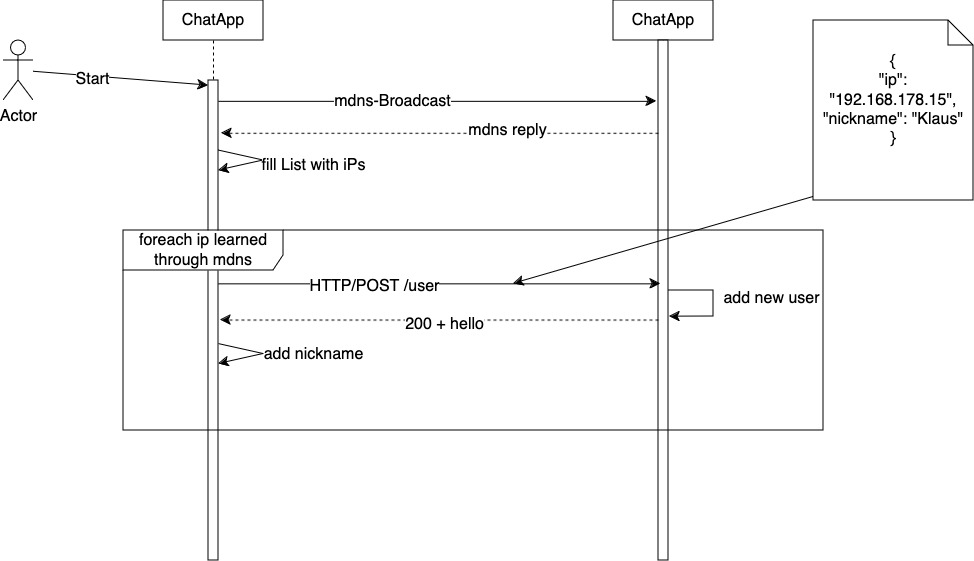
\includegraphics[scale=0.4]{Images/Initialisierung_Sequenzdiagramm.jpg}
    \captionbelow{Initialisierung}
\end{figure} 
\\
Nachdem man dem Chatroom beigetreten ist können Nachrichten verschickt werden. Abbildung 2 zeigt wie die Kommunikation und das Versenden von Nachrichten abläuft.
Der User schreibt eine Nachricht. 
Um diese Nachricht zu verschicken muss der Client in der Userliste alle IP Adressen der Teilnehmer nachschauen. Die Nachricht wird anschließend 
an jede einzelne IP Adresse geschickt. Das Versenden der Nachrichten findet ebenfalls mittels HTTP statt.
\begin{figure}[h]
    \centering
    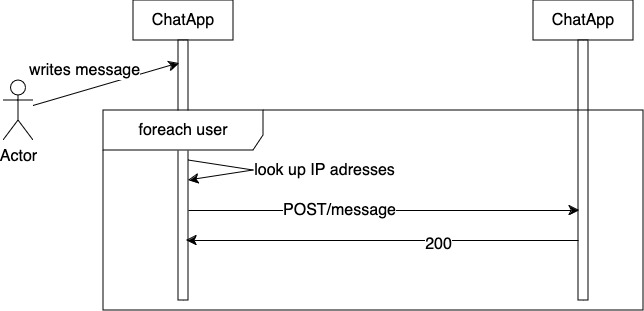
\includegraphics[scale=0.4]{Images/Kommunikation_Sequenzdiagramm.jpg}
    \captionbelow{Kommunikation}
\end{figure}
\\
Soll das Programm beendet werden und man möchte aus dem Chatroom austreten, müssen die anderen Teilnehmer informiert werden, dass man nicht mehr im Chatroom teilnimmt.
Wenn das Programm beendet wird, werden trotz des Austritts weiterhin Nachrichten an die Adresse geschickt, obwohl dieser Teilnehmer den Chatroom verlassen hat, da die Adresse weiterhin in der Userliste steht.
Um zu verhindern, dass Ressourcen verschwendet werden und ein Teilnehmer nach seinem Austritt auch keine weiteren Nachrichten mehr erhält, wird eine Exitmessage benötigt. Diese kündigt an, dass der Teilnehmer nun 
den Chatroom verlässt und keine Nachrichten mehr bekommen soll. 
Wie in Abbildung 3 zu sehen ist, wird beim Verlassen des Chatrooms wieder über HTTP eine Exitmessage an alle Teilnehmer gesendet. Die Exitmessage enthält wie die Startmessage den eigenen Namen und die IP Adresse.
Der User wird von den anderen Teilnehmern aus der Userliste entfernt und der Client ist somit dem Chatroom ausgetreten. 
\begin{figure}[h]
    \centering
    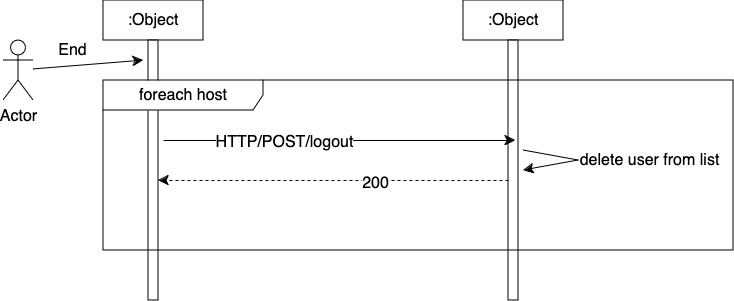
\includegraphics[scale=0.4]{Images/Exit_Sequenzdiagramm.jpg}
    \captionbelow{Exit}
\end{figure}
\newpage